\setcounter{part}{1}

\chapter{Contexte}
	\setcounter{chapter}{1}
	\section{SensioLabs}



	\section{Blackfire}

\begin{figure}[!h]
\begin{center}
    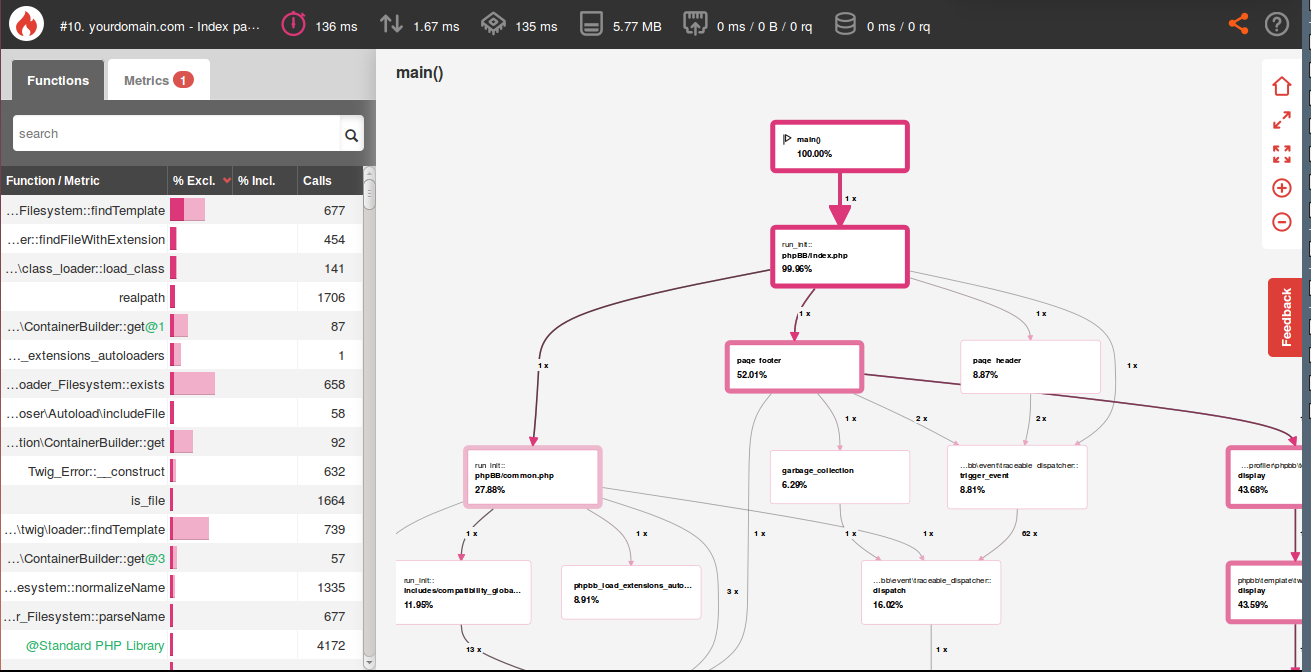
\includegraphics[width=0.8\textwidth]{images/blackfire-exemple}
  %\vspace{-22pt}
  \caption{Exemple de profile généré par \Blackfire}
  \centering
\end{center}
\end{figure}

Dernier outil développé par l'équipe produit de \SensioLabs, \Blackfire\footnote{\url{https://blackfire.io}},
sorti commercialement le 27 juillet 2015 après une année de béta test publique, est un produit disponible en mode \gls{SAAS} permettant d'analyser les performances d'applications \PHP de manière simple, précise et juste.

\Blackfire fourni un moyen pour instrumenter automatiquement un code \PHP existant afin d'en extraire des données telle que le \gls{graphe d'appels} du programme ou le temps passé dans chaque fonction et de les représenter sous une forme graphique intuitive permettant ainsi au développeur d'identifier les principaux problèmes de performance de son application.\footnote{Voir chapitre \vref{chap:Blackfire} pour plus de détails sur \Blackfire et son fonctionnement}

%	\section{Python}
% TODO Voulons nous vraiment parler de Python dans le contexte ?
% \Python est un langage de programmation 

\chapter{Objectifs}
	\setcounter{chapter}{2}
	
\begin{figure}[!h]
\begin{center}
  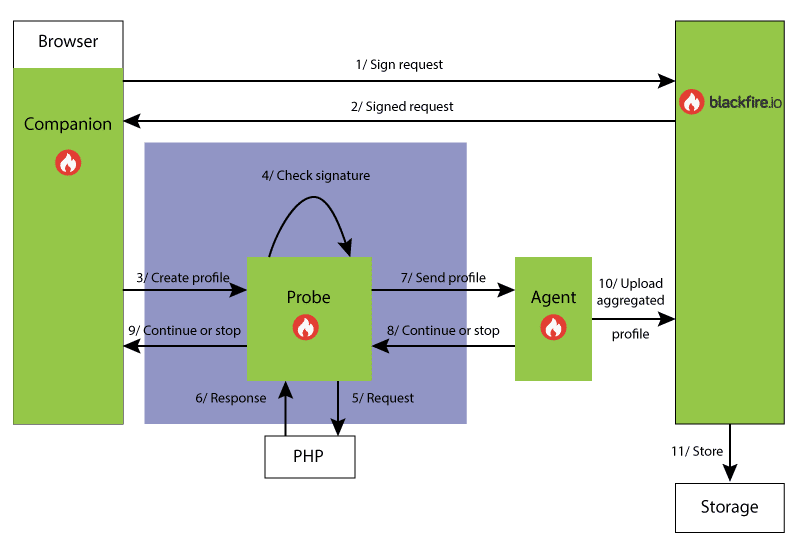
\includegraphics[width=0.8\textwidth]{images/schemas/workflow/general-workflow}
  \caption{Organisation générale de \Blackfire}
  % TODO remplacé par le même schéma en simplifié (moins de flèches. le but est de montrer les composants et qui utilise quoi)
\end{center}
\end{figure}

\Blackfire est organisé en 4 composants communiquant les uns avec les autres:
\begin{itemize}
\item Le compagnon, disponible dans Chrome sert à déclencher l'analyse
\item \textbf{blackfire.io} est le site web qui affiche les résultats
\item L'agent fait le liens entre la sonde et le site blackfire.io
\item La sonde est branchée sur le programme de l'utilisateur et collecte des données
\end{itemize}

Les 3 premiers composants ont étaient conçus de manière à être génériques et devraient donc être capables de traiter avec des données issues de n'importe quelle technologie du moment que le protocole\footnote{Voir section \vref{sec:BlackfireProtocol}} est respecté. Et en pratique il est effectivement possible d'afficher via \textbf{blackfire.io} des profiles générés via d'autres outils tel que Callgrind\footnote{\url{http://blog.blackfire.io/cli-upload.html}}, Google Chrome JavaScript CPU profiles\footnote{\url{http://blog.blackfire.io/chrome-cpu-profiles.htmll}} et bien d'autres\footnote{\url{http://blog.blackfire.io/profiling-web-page-loading-performance.html}}\footnote{\url{http://blog.blackfire.io/blackfire-file-format.html}}.

Mais le principal problème d'utiliser ces outils c'est que l'on a pas la même expérience que lorsque on profile un code \PHP avec \Blackfire. En effet, n'utilisant pas \Blackfire pour collecter les données on ne peut pas utiliser le compagnon pour déclencher un profile en 1 clic, l'impact de la collecte des données sur les performances peut être important et surtout l'expérience utilisateur peut être compliqué : on peut être obligé d'instrumenter manuellement son code et une fois le profile générer il faut encore le convertir dans le format utilisé par \Blackfire et l'uploader.

L'enjeu est multiple, il s'agit d'une part de démontrer que la plate-forme \Blackfire est effectivement générique (et le cas échéant de corriger dans la plate-forme ou le protocole les différents problèmes qui empêchent ou gênent cette généricité) et d'autre part d'apporter le support du langage \Python.

L'objectif est donc de réaliser une nouvelle implémentation de la quatrième partie, la sonde, qui serait capable d'analyser des programmes \Python avec une expérience utilisateur la plus proche possible de celle que l'on a actuellement avec la sonde \PHP, ce qui implique que la sonde doit :
\begin{itemize}
  \item permettre d'analyser du code \Python\footnote{Ce qui implique à minima le graphe d'appel du programme et le temps passé dans chaque fonction/méthode}
  \item communiquer avec l'\gls{agent} en respectant le protocole
  \item avoir un impact (\gls{overhead}) minimal\footnote{Afin de garantir des résultats aussi fidèles à la réalité que possible}
  \item instrumenter le code automatiquement
  \item ne déclencher l'analyse qu'à la demande\footnote{De cette manière la sonde peut être déployée en production}
\end{itemize}

\setcounter{part}{0}
\setcounter{chapter}{0} 